\subsubsection{Attitude Controller Simulation}
In the following section the final design of the attitude controller is given. Hence the final pole locations from the state feedback and the observer are provided. The final angle response, step response of the angles and observer estimation of the attitude controller can therefore be analysed and discussed. To be able to discussed the final result and illustrate the iteration process which has been used to find the final pole locations, the state feedback and observer are changed. Thus it is possible to yield reasoning for why the final design of the attitude controller is as it is.

A short description for the following three figures, \autoref{fig:ssFinalEq}, \autoref{fig:ssObsFinal} and \autoref{fig:ssFinalStep}, which is the final angle response, step response and the estimation of the angular velocities, is given. The weighted matrices, $\vec{Q_{final}}$ and $\vec{R_{final}}$, and the observer gain, $\vec{L_{obs}}$, which is utilized for the final attitude controller can be seen in \autoref{app:matricesSS}.

In \autoref{fig:ssFinalEq} a simulated angle response of the final attitude controller is shown. Initial conditions at time zero are given to the three angles. These are set to $0.2$ radians for the pitch, $-0.3$ for the roll and $-0.2$ for the yaw. The reference which the three angles is set to converge to is zero. \\ It can be seen from the figure that it approximately takes $2.5$ seconds for the pitch and roll to settle at zero, where it only takes approximately $1.4$-$1.5$ for the yaw.
%
\begin{figure}[H]
	\centering
	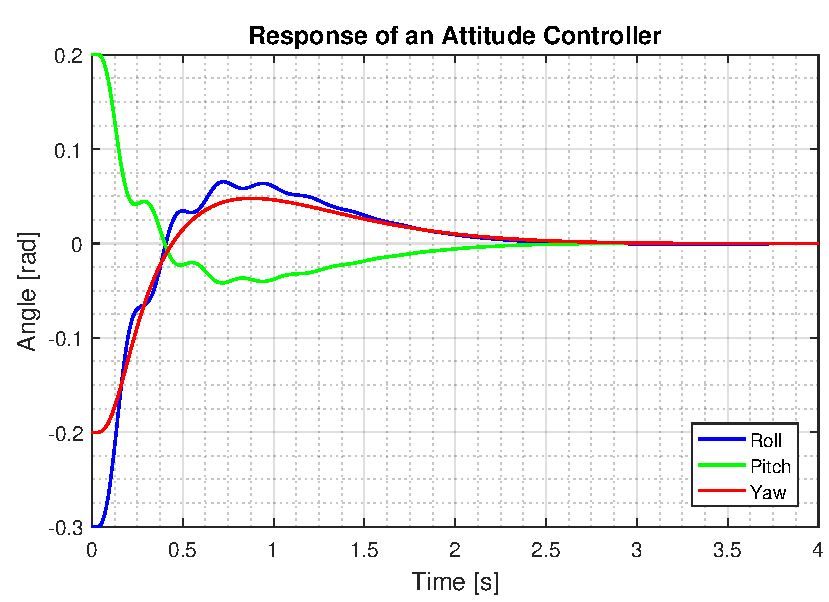
\includegraphics[scale=0.8]{figures/ssFinalEq.pdf}
	\caption{System response of the attitude controller, with initial conditions of $0.2$ radians for the pitch, $-0.3$ radians for the roll and $-0.2$ radians for the yaw. The weighted matrices, $\vec{Q_{final}}$ and $\vec{R_{final}}$, and the observer gain, $\vec{L_{obs}}$, which are utilized for the final design can be seen in \autoref{app:matricesSS}.}
	\label{fig:ssFinalEq}
\end{figure}
%
In \autoref{fig:ssObsFinal} the observer estimation for the angular velocity in roll, pitch and yaw is shown. The simulation is related with the angle response shown in \autoref{fig:ssFinalEq}, as the utilized initial conditions are identical. To be able to evaluate the observers estimation (the red line), the actual angular velocity is illustrated as well (the blue line). \\ Differences between the actual angular velocity and the estimated can be seen. The estimations large spikes in the beginning of the three figures are due to the initial conditions for the angles. As the observer utilizes the angles for the estimation of the angular velocities \autoref{sec:AttitudeControllerDesign}. \\ The large gap between the actual and the estimation, could be due to multiple factors. First, the delay in the system, which is the sampling rate at $35$ \si{ms} \autoref{chap:Control}. Furthermore the observer utilizes the created model for the quadcopter, see \autoref{chap:Model}. As the model is not a perfect replica of how the system behaves in reality, errors are unavoidable. The small triangular spikes are both due to the sampling rate and the integrator in the observer. Each time the observer receives new angles the steep increase or decrease occur. As there is an integrator in the observer the estimation either decreases or increases until new angles arrives $35$ \si{ms} later.
%
\begin{figure}[H]
	\centering
	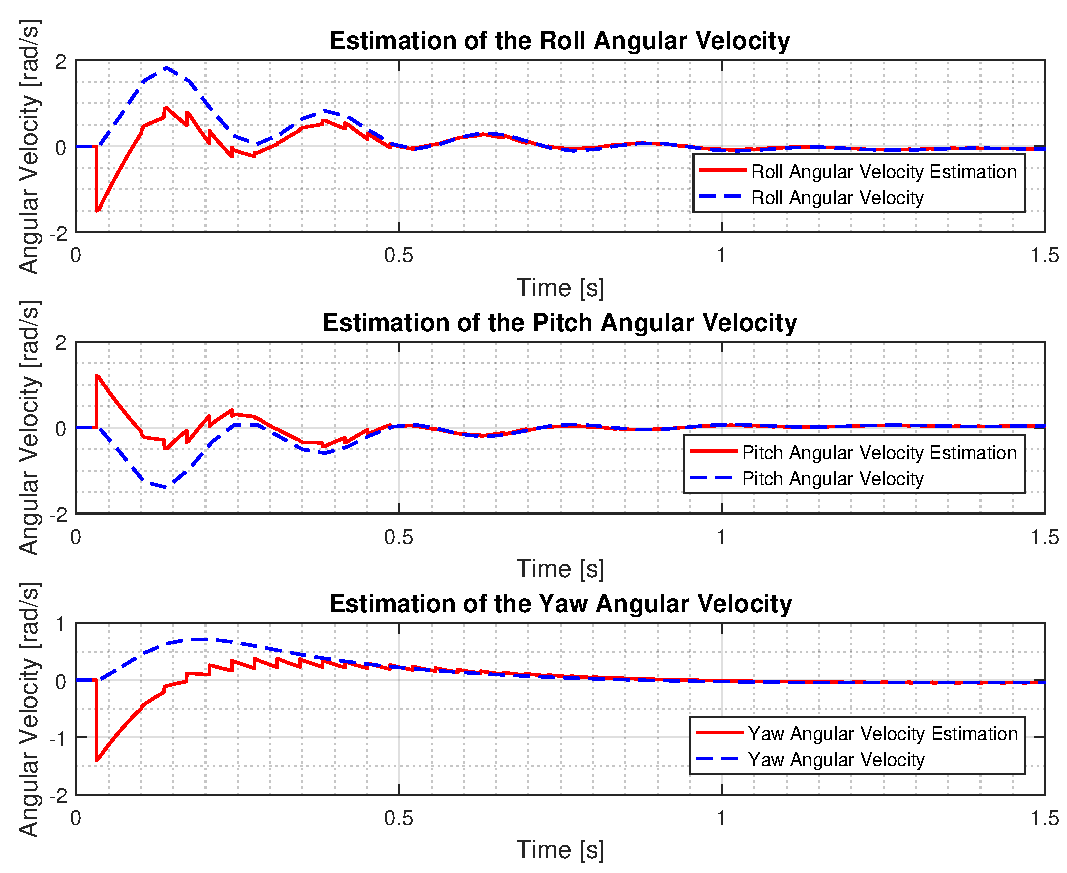
\includegraphics[scale=0.7]{figures/ssObsFinal.pdf}
	\caption{The three figures shows the estimation of the angular velocities made by the implemented observer. The simulations initial conditions for roll, pitch and yaw are identical to the simulation in \autoref{fig:ssFinalEq}. The utilized weighted matrices, $\vec{Q_{final}}$ and $\vec{R_{final}}$, and the observer gain, $\vec{L_{obs}}$, can be found in \autoref{app:matricesSS}.}
	\label{fig:ssObsFinal}
\end{figure}
%
A step response of the roll and pitch, with a reference set to one, is shown in \autoref{fig:ssFinalStep}. The yaw is not illustrated as the reference is consistently set to zero, see \autoref{chap:Control}. It is therefore only desired to discover how the roll and pitch responds to a reference shift. It can be seen that the step response of the two angles is similar, this is expected as the implementation of the two is identical. \\ With an error band of 5 percent, the settling time is approximately $1.5$ \si{s} and the overshoot is less than 5 percent. 
%
\begin{figure}[H]
	\centering
	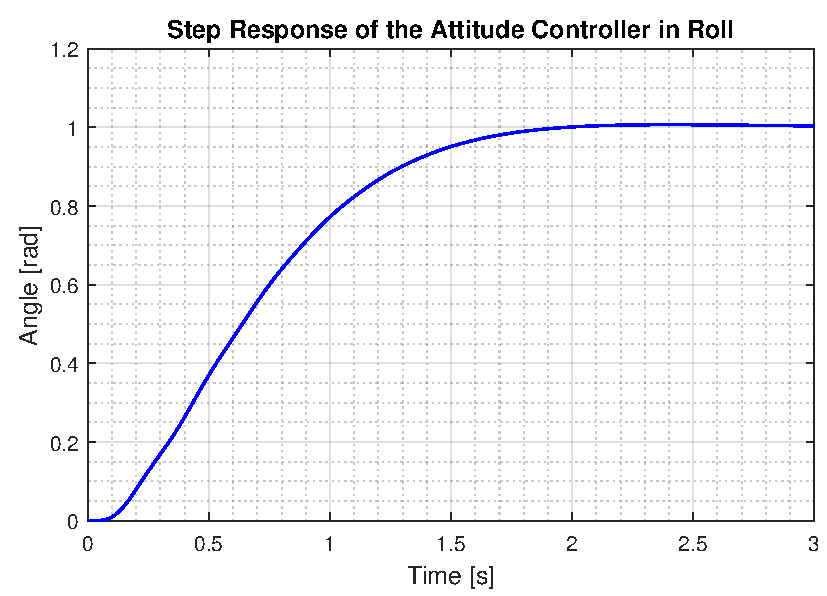
\includegraphics[scale=0.8]{figures/ssFinalStep.pdf}
	\caption{An step response of the final system. This illustrates only the behavior of the roll and the pitch, as the yaw is always set to zero. The utilized weighted matrices, $\vec{Q_{final}}$ and $\vec{R_{final}}$, and the observer gain, $\vec{L_{obs}}$, can be found in \autoref{app:matricesSS}.}
	\label{fig:ssFinalStep}
\end{figure}
%
The final system design has been analysed and shown. To illustrate the iterative process utilized to find the final weighted matrices and observer gain a few simulations are shown. Only one parameter for each simulation is changed at a time. It is thereby possible to compare and discuss the different simulation to the final design and why the final parameters has been chosen.

The weighted matrices utilized for the simulation, in \autoref{fig:TranslationalControlDiagram}, are changed relative to the final design. The new matrices called $\vec{Q_{high}}$ and $\vec{R_{high}}$ can be seen in \autoref{app:matricesSS}. Compared to the final design the allow state error in the angles is less and the allow control action is increased. These changes should yield a more reactive system. This can be seen in the angle response shown in \autoref{fig:TranslationalControlDiagram}. Note that the initial conditions for the response are similar to \autoref{fig:ssFinalEq}.

It can be seen from \autoref{fig:TranslationalControlDiagram} that by changing the weighted matrices relative to the final design, the roll begins to oscillate. As there is a delay in the system and the system is set to react faster, the controller is not able to stabilize the roll. Since the absolute value for the initial conditions for roll is larger than the pitch, it is the roll which is oscillating. From this it is possible to conclude that a higher feedback gain compared to the final is not desired for the attitude control.
%
\begin{figure}[H]
	\centering
	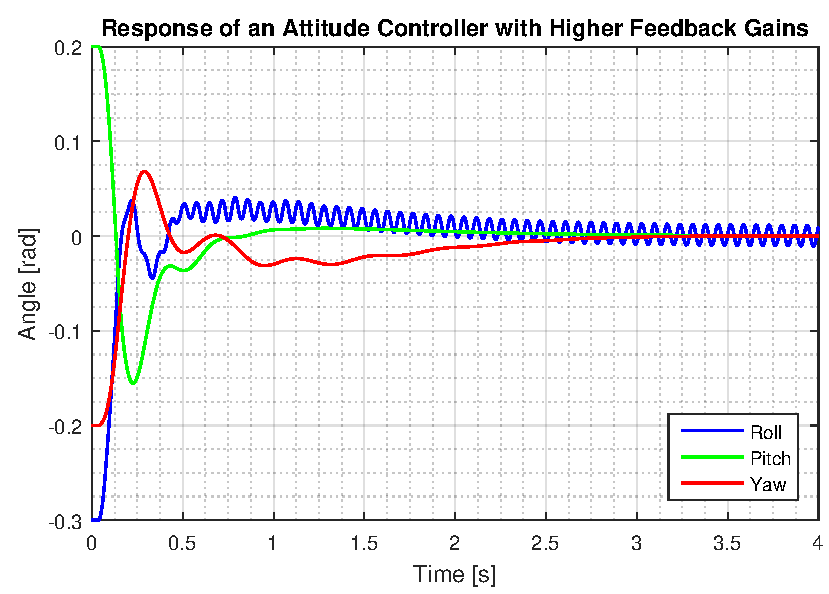
\includegraphics[scale=1]{figures/ssEqBad.pdf}
	\caption{The simulation is generated by utilizing the weighted matrices, $\vec{Q_{high}}$ and $\vec{R_{high}}$, and the observer gain, $\vec{L_{obs}}$, found in \autoref{app:matricesSS}. The initial conditions for the angles is set to $0.2$ radians for the pitch, $-0.3$ radians for the roll and $-0.2$ radians for the yaw.}
	\label{fig:TranslationalControlDiagram}
\end{figure}
%
The observer gain, $\vec{L_{obsH}}$, utilized for the simulation in  \autoref{fig:TranslationalControlDiagram} is increased compared to the gain utilized in the final design. This results in more oscillations from both the pitch and the roll. Additionally, the yaw takes more time to settle compared to the final design, shown in \autoref{fig:ssFinalEq}. It is evident that when increasing the gain the observer is worse at estimating the angular velocity compared to the final design.
%
\begin{figure}[H]
	\centering
	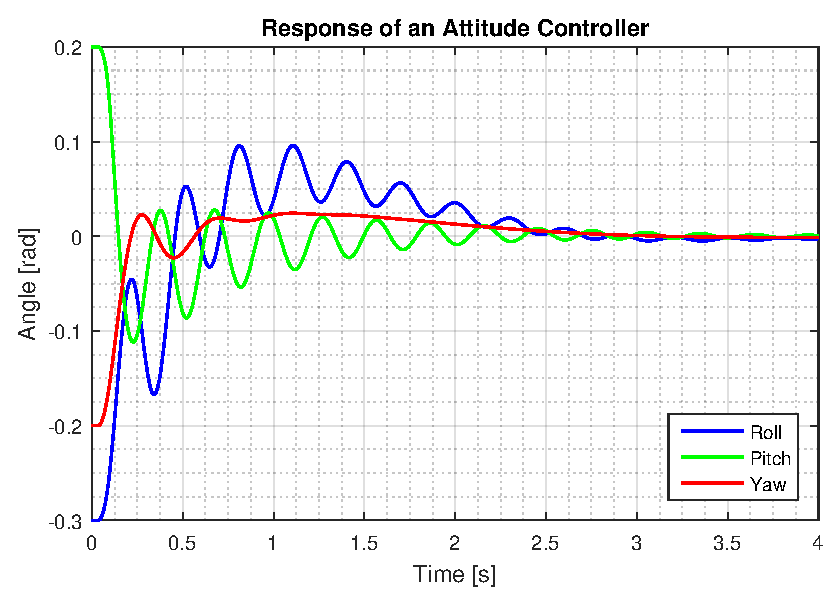
\includegraphics[scale=0.8]{figures/ssEqObsHigh.pdf}
	\caption{Simulation illustrating an angle response with an increase in the observer gain compared to the final design. The utilized weighted matrices, $\vec{Q_{final}}$ and $\vec{R_{final}}$, and the observer gain, $\vec{L_{obsH}}$ can be found in \autoref{app:matricesSS}.}
	\label{fig:TranslationalControlDiagram}
\end{figure}
%
From the simulations in \autoref{fig:TranslationalControlDiagram} and \autoref{fig:TranslationalControlDiagram} it is evident that an increase in gain in either the state feedback or in the observer is not desired compared to the final design.\\ The final design made with a compromise between a fast system, with a lot of oscillating behavior, and a slow system without oscillating behavior. \\ The Attitude controller has been design and simulated, it is now possible to look into the design of the translational controller.


